\documentclass[11pt, conference, letterpaper]{IEEEtran}
\usepackage[utf8]{inputenc} % set input encoding (not needed with XeLaTeX)
%\usepackage{geometry}
%\geometry{letterpaper}
%%% Examples of Article customizations
% These packages are optional, depending whether you want the features they provide.
% See the LaTeX Companion or other references for full information.



\usepackage{graphicx} % support the \includegraphics command and options

% \usepackage[parfill]{parskip} % Activate to begin paragraphs with an empty line rather than an indent

%%% PACKAGES
\usepackage{url}
\usepackage{booktabs} % for much better looking tables
\usepackage{array} % for better arrays (eg matrices) in maths
\usepackage{paralist} % very flexible & customisable lists (eg. enumerate/itemize, etc.)
\usepackage{verbatim} % adds environment for commenting out blocks of text & for better verbatim

\usepackage{subcaption}
%\usepackage{subfig} % make it possible to include more than one captioned figure/table in a single float
\usepackage{algorithm} 
\usepackage{algorithmic}
\usepackage{amsmath}
\usepackage[font=small]{caption}
\usepackage{afterpage}



% These packages are all incorporated in the memoir class to one degree or another...

%%% HEADERS & FOOTERS
%\usepackage{fancyhdr} % This should be set AFTER setting up the page geometry
%\pagestyle{fancy} % options: empty , plain , fancy
%\renewcommand{\headrulewidth}{0pt} % customise the layout...
%\lhead{}\chead{}\rhead{}
%\lfoot{}\cfoot{\thepage}\rfoot{}

%%% END Article customizations

%%% The "real" document content comes below...

\title{VHash: An Optimized Voronoi-Based Distributed Hash Table}
%\author{Double Blind}
%\author{Brendan Benshoof \qquad Andrew Rosen  \\Department of Computer Science, Georgia State University\\  bbenshoof@cs.gsu.edu \qquad rosen@cs.gsu.edu }
\date{} % Activate to display a given date or no date (if empty),
         % otherwise the current date is printed 

\begin{document}
\maketitle

\begin{abstract}
%1. State the problem
Distributed Hash Tables (DHT) provide a fast and robust decentralized means of key-value storage and retrieval and are typically used in Peer-to-Peer applications.
DHTs assign nodes a single identifier derived from the hash of their IP address and port, which results in a random overlay network.   
%2. Say why it’s an interesting problem
A random overlay network is not explicitly optimized for certain metrics, such as latency, energy, or hops on an overlay network. 
Being able to do so will allow for tighter control over the network behavior and enable higher performance DHT applications.
%It is often desirable to generate an overlay network that is optimized for one or more specific metrics.

%3. Say what your solution achieves
This paper presents VHash, a DHT protocol to construct an overlay optimized for such metrics. 
VHash exploits a fast and efficient Delaunay Triangulation heuristic to approximate Voronoi regions in a geometric space. 
%4. Say what follows from your solution
We used VHash to generate an overlay with edges that minimize latency. 
While we focused on latency in this paper, VHash optimizes on any defined metrics.
This approach outperforms overlays generated by the Chord DHT protocol in terms of lookup time.
VHash provides a robust, scalable, and efficient distributed lookup service.

\end{abstract}
%  We could use a different config 
% networks are only hpped
% we can do non-euclidean metrics if we have a non-euclidean distance and midpoint definition


\section{Introduction}


Voronoi graphs \cite{voronoi} have been  a topic of interest for distributed and  peer-to-peer (P2P) applications for some time now.
Voronoi graphs can be used as part of distributed hash tables\cite{virtvoro}
Coverage detection \cite{carbunar2004distributed}

MMOs \cite{hu2008voronoi} \cite{Backhaus:2007:VAS:1326257.1326266}


Computing the Voronoi graph is a well known problem and has many algorithms to compute the Voronoi regions with complete, global knowledge.

Network applications are distributed and need to have a distributed means of doing this computation

Finally, we run into trouble when we get to >2 dimensions.
$O(n^{\frac{2d-1}{d}}) $ \cite{watson1981computing}

Distributed networks are designed to be fault0-tolerant and can accept a margin of error.  
It makes sense to use heuristics instead


We have a quick new heuristic.


\section{Distributed Greedy Voronoi Heuristic}
The Distributed Greedy Voronoi Heuristic (DGVH) is a fast method for nodes to select peers from their Deluanay Triangulation (Algorithm \ref{DGVH}).
The rationale for this heuristic is that, in the majority of cases, the midpoint between to nodes falls on the common boundary of their Voronoi regions.

\begin{algorithm} % make smaller
\caption{Distributed Greedy Voronoi Heuristic}
\label{DGVH}
\begin{algorithmic}[1]  % the numberis how many lines
	 \STATE Given node $n$ and its list of $candidates$.
   	 \STATE Given the minimum $table\_size$
    \STATE $short\_peers \leftarrow$ empty set of $n$'s one-hop peers
	 \STATE $long\_peers \leftarrow$ empty set of $n$'s two-hop peers    
    \STATE Sort $candidates$ in ascending order by each node's distance to $n$
    \STATE Remove the first member of $candidates$ and add it to $short\_peers$
    \FORALL{$c$ in $candidates$}
    	\STATE $m$ is the midpoint between $n$ and $c$
        \IF{Any node in $short\_peers$ is closer to $m$ than $n$}
        	\STATE Reject $c$ as a peer
        \ELSE
        	\STATE Remove $c$ from $candidates$
        	\STATE Add $c$ to $short\_peers$
        \ENDIF
    \ENDFOR
    \WHILE{$|short\_peers| < table\_size$ \AND $|candidates| >0$}
    	\STATE Remove the first entry $c$ from $candidates$
    	\STATE Add $c$ to $short\_peers$
    \ENDWHILE
    	\STATE Add $candidates$ to the set of $long\_peers$	
    	\IF{$|long\_peers| > table\_size^2$}
        		\STATE $long\_peers \leftarrow$ random subset of $long\_peers$ of size $table\_size^2$
      \ENDIF
\end{algorithmic}
\end{algorithm}


Each cycle, nodes exchange their peer lists with a current neighbor and then recalculate their neighbors.  
A node combines their neighbor's peer list with its own to create a list of candidate neighbors.
This combined list is sorted from closest to furthest.
A new peer list is then created starting with the closest candidate.
The node then examines each of the remaining candidates in the sorted list and calculates the midpoint between the node and the candidate.
If any of the nodes in the new peer list are closer to the midpoint than the candidate, the candidate is set aside.  
Otherwise the candidate is added to the new peer list.

This heuristic has the benefit of being fast and scalable into any geometric space where a distance function and midpoint can be defined.
The distance metric used for this paper is the minimum distance in a multidimensional unit toroidal space.
Where $\vec{a}$ and $\vec{b}$ are locations in a $d$-dimensional unit toroidal space:
\[ distance = \sqrt{\sum\limits_{i\in d} (\min(|\vec{a}_i-\vec{b}_i|, 1-|\vec{a}_i-\vec{b}_i|))^2}\]


If a node is located between two other nodes, such that their midpoint does not fall upon the shared face of their Voronoi regions, then this heuristic will not link the blocked peers  (Figure \ref{occ-ex}).
Our algorithm handles these cases via our method of peer management.

\begin{figure}
	\centering
	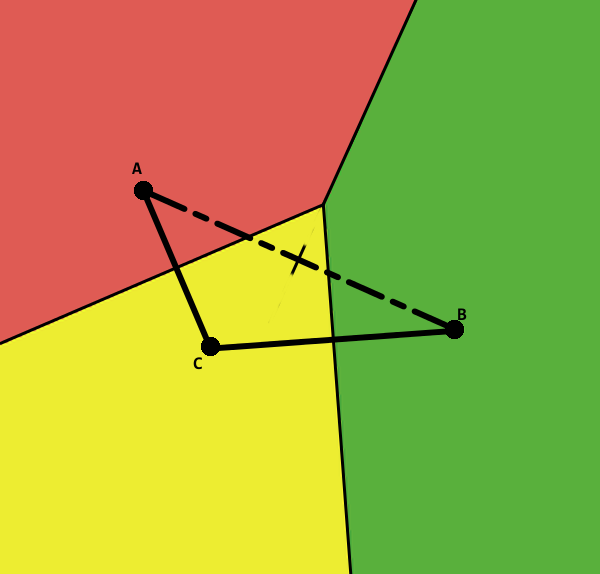
\includegraphics[width=\linewidth]{occlusion}
	\caption{The edge between $A$ and $B$ is not detected by DGVH, as node $C$ is closer to the midpoint than $B$ is.  This is mitigated by VHash's peer management polices.}  %Add labels a b c and reference the node labels in text
	\label{occ-ex}
\end{figure}

VHash never actually calculates the polytopes that describe a node's Voronoi region.
This is unnecessary and prohibitively expensive \cite{raynet}.
Rather, VHash assigns given points to their Voronoi regions.
It does this by calculating the distance from a given point to all candidate nodes.
The point falls into a node's Voronoi region if it is the node to which it has the shortest distance.
Thus a node defines its Voronoi region by keeping a list of the peers that bound it.


\section{Applications}


\section{Related Work}


\section{Conclusion}

\section{Introduction}
A Distributed Hash Table (DHT) protocol is used to provide an overlay network for many P2P applications. 
A DHT protocol allows peers to self organize and allocate responsibility for file distribution between each other \cite{bittorrent} \cite{kademlia} \cite{chord} \cite{pastry}.
Each peer in the network maintains a routing table of other peers in the overlay.
The configuration and rules of the routing table vary from one protocol to another.
However, they all have the common goal to minimize the number of overlay hops that a distributed lookup requires.
A routing table created to minimize overlay hops does not necessarily create routes with minimized overall network latency.

%In a DHT the entries of the routing tables may be separated by powers of 2 \cite{chord}, be determined by shared prefixes \cite{pastry}, or be chosen according to a probabilistic distribution \cite{kleinberg2000navigation}
 
We have designed a DHT protocol, VHash, that enables more sophisticated applications of DHTs to networking problems.
This paper shows that VHash generates an overlay network and routing method that not only reduces overlay hops, but also reduces actual latency across the underlying network as compared to existing DHTs.
%What if more information about the nodes could be encoded as part of the overlay, such as the node's latency?

DHTs are built on the premise of assigning locations in a geometric space to peers and files.
Peers are assigned areas in this space and are responsible for files and maintain connections with other peers accordingly.
Reducing latency in a DHT requires embedding a graph of inter-peer latency into such a geometric space.
This allows for efficient routing in the geometric space model and yields efficient routing on the network.

This requires solutions for two problems:
How do we create and maintain a DHT based on an arbitrary geometric space?
How do we usefully embed inter-node latency into the geometric space's coordinate system?

VHash provides a solution to both of these problems.
%VHash is designed to take inter-node latency information into account when generating an overlay.
VHash works in arbitrary geometric spaces by creating an approximate Voronoi partition and Delaunay Triangulation based on peer locations.
The Delaunay Triangulation defines the routing tables and the Voronoi partition dictates where content is stored in the network.
We accomplish this by assigning each node $d$ coordinates, rather than a single key.
We use a basic force directed model to embed the inter-node latency graph in the overlay and assign peer locations to reduce latency.
A result of this is that peers in VHash can \emph{move} through the metric space over the lifetime of the peer;  their position is not necessarily fixed and are expected to move as the network latency behavior changes.
%Other network metrics could easily be applied to VHash.

Our paper presents the following:
\begin{itemize}
	\item We describe the VHash protocol (Section \ref{vhash}) and the underlying approximation algorithm for Delaunay Triangulation and Voronoi regions.
    Our approximation is distributed, greedy, efficient, and accurate in an arbitrary number of dimensions.
     It creates an overlay with edges that minimize distance over network metrics while maintaining robustness, scalability, and polylogarithmic lookup time in overlay hops.
	\item We use VHash to provide us with an overlay for embedding network metrics.
    We present our force directed graph model for embedding nodes in the overlay with latency information (Section \ref{networkEmbedding}).% and discuss other network metrics that can be used with VHash (Section III).
	\item We present simulations (Section \ref{simSection}) to demonstrate that the overlays created by VHash enable routing messages from arbitrary source nodes to random destination locations efficiently.
    We also show that by embedding the latency graph, our routing dramatically outperforms DHTs that rely on $O(\lg(n))$ size routing tables, such as Chord \cite{chord}.
	\item We present related work upon which VHash is built and describe the improvements provided by VHash (Section \ref{related}).
	\item We discuss future work, including how VHash is capable of optimizing other network metrics beyond latency (Section \ref{conclusions}).
\end{itemize}

%\section{Background}
%\label{background}
%\subsection{Distributed Hash Tables}
%\subsection{Voronoi Regions and Delunay Triangulation}
%A Voronoi diagram is the partition of a space into cells or regions along a set of objects $O$ such that all the points in a particular region are closer to one object than any other object.  
%We refer to the region owned by an object as that object's Voronoi region.
%The Delaunay Triangulation of this same space along the same set of objects is defined by the edges such that no object is inside the circumcircle of any triangle formed by the edges \cite{geoalg}.  
%The Voronoi diagram and Delaunay Triangulation are dual problems, as an edge between two objects in a Delaunay Triangulation exists if and only if those object's Voronoi regions border each other.  
%This means that solving either problem will yield the solution to both.   An example Voronoi diagram is shown in Figure \ref{voro-ex}.


%\begin{figure}
%	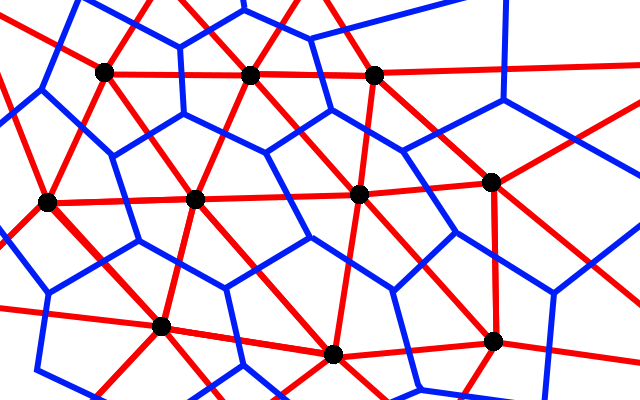
\includegraphics[width=\linewidth]{voronoi-example}
%	\caption{An example Voronoi diagram for objects on a 2-dimensional toroidal space.  The black lines correspond to the edges of the Delaunay Triangulation}.
%	\label{voro-ex}
%\end{figure}

%A formal and thorough description of Voronoi diagrams as well as their applications can be found in \cite{aurenhammer1991voronoi}.


\section{VHash}
\label{vhash}
This section presents the VHash DHT protocol to generate an overlay network topology.
VHash differentiates from other DHTs primarily in its method of peer selection.
Nodes in the VHash network periodically gossip with other nodes, exchanging locations of theirs peers and use an approximation algorithm to refine its list of neighbors.
These neighbors approximate the node's Voronoi region and its corresponding responsibilities.
A node is responsible for all data that is assigned to locations within its Voronoi region.
This approximation algorithm (Algorithm \ref{DGVH}) is fast and can be used in spaces with an arbitrary number of dimensions.

\subsection{Voronoi Regions in DHTs}
A Voronoi diagram is the partition of a space into cells or regions along a set of objects $O$ such that all the points in a particular region are closer to one object than any other object.  
We refer to the region owned by an object as that object's Voronoi region.
%This cleanly maps to the concept of ownership in DHTs, where nodes are responsible for n
%The Delaunay Triangulation of this same space along the same set of objects is defined by the edges such that no object is inside the circumcircle of any triangle formed by the edges \cite{geoalg}.  
The Voronoi diagram and Delaunay Triangulation are dual problems, as an edge between two objects in a Delaunay Triangulation exists if and only if those object's Voronoi regions border each other.  
This means that solving either problem will yield the solution to both.   An example Voronoi diagram is shown in Figure \ref{voro-ex}.
A formal and thorough description of Voronoi diagrams as well as their applications can be found in \cite{aurenhammer1991voronoi}.


\begin{figure}
	\centering
	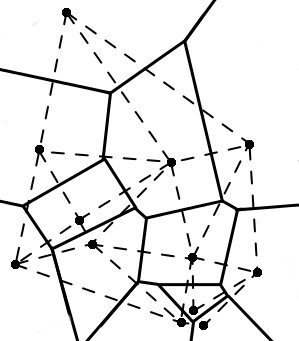
\includegraphics[width=0.75\linewidth]{voronoi}
	\caption{An example Voronoi diagram for objects on a 2-dimensional space.  The black lines correspond to the borders of the Voronoi region, while the dashed lines correspond to the edges of the Delaunay Triangulation}.
	\label{voro-ex}
\end{figure}


In our network, the nodes are the objects of the Voronoi diagram and are responsible for keys that fall in their region.
The edges created by the Delaunay Triangulation correspond to the connections between neighboring nodes. 
Computing Voronoi diagrams in a distributed and generalized fashion is prohibitively time expensive and previous work \cite{raynet} shows that an approximation is sufficient for peer selection and routing.
With VHash, we have created a new greedy, online algorithm that approximates and maintains the set of peers defining the node's Voronoi region and Delaunay Triangulation.

Arguably all DHTs are built on the concept of Voronoi regions.
In all DHTs a node is responsible for all points in its hash space to which it is the ``closest'' node.
These DHTs have carefully chosen metric spaces such that these regions are very simple to calculate.
For example, Chord and similar ring-based DHTs utilize a unidirectional, one-dimensional ring as their metric space, such that the region for which a node is responsible is the region between itself and its predecessor.
VHash generalizes these same behaviors: by choosing a particular metric space, VHash can approximate other DHTs.
The toroidal metric space utilized in this paper is an extension of the ring topology used by Chord \cite{chord}, Symphony \cite{manku2003symphony}, and others into additional dimensions. 

The cost of generalizing VHash to utilize any geometric space is the efficiency of calculating Voronoi regions. 
It is prohibitively expensive to generate an exact calculation of the Deluanay peers and Voronoi regions of a geometric space in a distributed fashion \cite{raynet}.  %\footnote{They cite Geometric Algorithms by Boissonat}. 
Previous explorations into distributed approximations of a node's Voronoi region offer constant time approximations.
The greedy heuristic we use is approximately as fast as a single sample calculation in the Monte-Carlo approach used in RayNet \cite{raynet}.
As a heuristic, there exist edge cases where it is incorrect.
We show in the experimental section that this loss in accuracy has no practical impact.

\subsection{Distributed Greedy Voronoi Heuristic}
%snip
\subsection{Peer Management}
VHash maintains two peer lists: \textit{Short Peers} and \textit{Long Peers}.
This is motivated by mitigating the error induced by DGVH and providing robustness against churn\footnote{The disruption caused to the overlay by the continuous joining, leaving, and failing of nodes.}.

\textit{Short Peers} are the subset of the Delaunay Peers generated by DGVH. 
The number of short peers has no upper bound and in contrived cases, such as a single node surrounded by other nodes forming a hypersphere, it can grow quite high.
Previous work has found a useful lower bound on peers to be $3d + 1$ \cite{raynet}.
Using a lower bound on the length of the short peer list corrects for errors in the approximation processes by including peers that would otherwise be omitted. 
$3d+1$ is used as the lower bound for the size of the short peer list.
Should the number of short peers generated by DGVH be less than the lower bound for that set's size, the nearest peers not already included in the short peer list are added to the short peer list, until it is of sufficient size.
Members of \textit{Short Peers} are analogous to the predecessors/successors in other DHTs.

\textit{Long Peers} is the list of two-hop neighbors of the node.
When a node learns about potential neighbors, but are not included in the short peer list, they may be included in the long peer list.  
The long peer list has a maximum size of $(3d+1)^2$.  
For example, if the short peer list has a minimum size of 8, the long peer list has a maximum size of 64 entries.  
Members of \textit{Long Peers} are not actively probed during maintenance and the cost of managing them is minimal.

We next discuss how nodes learn about short and long peers.

\subsection{Maintenance via Gossiping}
Each node in the network performs maintenance periodically by `gossiping' with a randomly chosen neighbor.
When two nodes gossip with each other, they exchange their short peer lists with each other.
The node combines the lists of short peers\footnote{Nodes remove themselves and repetitions from the candidates.} and uses DGVH to determine which of these candidates correspond to its neighbors along the Delaunay Triangulation.
The candidates determined not to be short peers become long peers.  
If resulting number of long peers exceeds the maximum size of the long peer list, a random subset of the maximum size is kept.

The formal algorithm for this process is described in Algorithm~\ref{gossip}.
This maintenance through gossip process is very similar to the gossip protocol used in \cite{raynet}.


\begin{algorithm}
\caption{Gossiping}
\label{gossip}
\begin{algorithmic}[1]  % the number is how many 
	\STATE Node $n$ initiates the gossip.
	\STATE $neighbor \leftarrow$ random node from $n.short\_peers$
   \STATE $n\_candidates \leftarrow n.short\_peers \cup n.long\_peers \cup neighbor.short\_peers$
   \STATE $neighbor\_candidates \leftarrow neighbor.short\_peers \cup neighbor.long\_peers \cup n.short\_peers$.  
   \STATE $n$ and $neighbor$ each run Distributed Greedy Voronoi Heuristic using their respective $candidates$
\end{algorithmic} 
\end{algorithm}



\subsection{Handling Churn}
Churn refers to the effects caused by the continuous joining and exiting of nodes to and from the overlay.
DHTs must have some mechanisms to handle this process to maintain fault tolerance and accurate routing as their members change over time.

Joining the VHash network is a straightforward process.  
A prospective node must be able to communicate with at least one patron member of the DHT.  
The prospective node is assigned a location using the method described in Section \ref{networkEmbedding} and uses the patron to find the node responsible for its assigned location, which we call the parent.
The prospective node sets the parent node as the lone member of \textit{Short Peers} and immediately gossips with the parent.
Subsequent gossips will refine the peer lists of the nodes affected by the join.


There is no ``polite'' method of leaving the network. 
VHash assumes nodes will fail often and abruptly and that the distinction between an intended failure and unintended failure is unnecessary.
Should a node wish to leave the network, it only needs to cease sending and receiving messages.
Suppose a node $f$ fails or leaves the network; we assume it does so without warning.
When one of $f$'s neighbors attempts to contact $f$ for gossiping or routing, failure to communicate with $f$ will prompt the neighbor to remove $f$ from its peers.  
The node then selects a different neighbor to gossip with or recomputes the peer closest to the location it was looking for. 
Should a short peer fail, routing around its failure is trivial due to knowledge about the long peers.


\subsection{Routing}
The proper forwarding peer for routing a message extends from the Voronoi regions of \textit{Short Peers}and \textit{Long Peers}.
For the purposes of routing, each node assumes itself and its short and long peers are the only nodes that exist in the geometric space.  
When a node receives a message destined for a particular location, that node determines whether or not it is closest to that location.
This is the same as determining whether or not the specified location falls into the node's Voronoi region.
If this is the case, the node handles the message accordingly.  
Otherwise, one of its peers must be responsible for that location.
It forwards the message to the peer it deems closest to the location, which repeats the same decision process, but with different knowledge.

%Rather than attempt to know the true Voronoi region of those peers, we approximate the Voronoi regions of those peers as if there where no other nodes in the network.
%The resulting voronoi regions describe both the subset of the network for which that peer is responsible and the subset of the network for which it is the most efficient forwarding node.
%The routing node determines the voronoi region into which the message's destination falls.
%If this is itself, it handles the message accordingly; otherwise the routing node forwards the message to the responsible node.
This process is equivalent to a precomputed, cached, and efficient routing algorithm (Algorithm \ref{lookup}), shown to be polylogarithmic by \cite{raynet} \cite{kleinberg2000navigation} \cite{voronet}.
In the case that our approximation of the Voronoi region of a peer is incorrect due to each nodes incomplete knowledge of the network, our approximation describes the most efficient forwarding path of a message to a particular location.

\begin{algorithm}
\caption{VHash Lookup}
\label{lookup}
\begin{algorithmic}[1] 
	\STATE Given node $n$
	\STATE Given $m$ is a message addressed for $loc$
    \STATE $potential\_dests \leftarrow n \cup n.short\_peers$
    \STATE $c \leftarrow $ node in $ potential\_dests$ with shortest distance to $loc$
    \IF{$c$ == $n$}
    	\RETURN $n$
    \ELSE
        \RETURN $c.lookup(loc)$
    \ENDIF
\end{algorithmic}
\end{algorithm}



\subsection{Algorithm Analysis}
DVGH is very efficient in both terms of space and time.  
Suppose a node $n$ is creating its short peer list from $k$ candidates in an overlay network of $N$ nodes. 
The candidates must be sorted, which takes $O(k\cdot\lg(k))$ operations.  
Node $n$ must then compute the midpoint between itself and each of the $k$ candidates.  
Node $n$ then compares distances to the midpoints between itself and all the candidates.  
This results in a cost of 

\[ k\cdot\lg(k) + k \text{ midpoint computations}  + k^{2} \text{ distance computations} \]


Since  $k$ is  bounded by $\Theta(\frac{\log N}{\log \log N} )$ \cite{bern1991expected} (the expected maximum number of peers stored between two neighbors), we can translate the above to

\[O(\frac{\log^{2} N}{\log^{2} \log N} )\]

In the vast majority of cases, the number of peers is equal to the constant minimum table size. This yields $k=(3d+1)^2+3d+1$ in the expected case, where the lower bound and expected complexities are $\Omega(1)$.

Previous work \cite{raynet} claims constant time approximation, the reality is that Raynet's leading constant is in the order of thousands as Monte-Carlo samples.  
Our algorithm has a greater asymptotic worst case cost, for all current realistic network sizes it will be more time efficient then RayNet's approximation.






\section{Network Metric Embedding}
%Describe initial location assignment
\label{networkEmbedding}
During previous research in applications of DHTs \cite{andrew-poster} to parallel processing, Rosen et al.\ tested DHT network behavior under churn. 
They came to the conclusion that high levels of churn improved the performance of the system under certain circumstances.
The built-in mechanisms for managing responsibility in a DHT are very effective and efficient at handling nodes changing locations in the network.
In this work, Rosen et al.\ found that it was more effective to move the node to a location in the DHT where work or data was stored rather than attempt to remap data efficiently over the nodes.

VHash is designed to leverage this discovery and allow a nodes' location in the network to provide meaningful information about the node and to allow nodes to change location in the network to suit the networks needs.
In this paper we propose a method that enables peers to periodically change their location in the network such that routes taken on the resulting overlay network have lower latency than would otherwise possible in a DHT.
Each node is given a random initial location and, over time, migrates to a location which optimizes latency.


We utilize a distributed, online graph embedding algorithm to find locations in the coordinate system for each node such that the latency between nodes can be accurately represented.
Once inter-node latency is effectively represented as distance in the coordinate space, routing for shortest distance across this space also routes along the shortest latency path on the overlay network.

For our simulations, we measure latency in terms of hops on a large scale free graph (10,000 nodes) that acts as an underlying network.
We simulate a small fraction of these nodes to act as members of a DHT and simulate VHash's and Chord's distributions of latency for recursive lookups.
Each node in the network performs a periodic update step to its location to accurately represent inter-node latency on the coordinate system.
We utilize a toroidal metric space for these experiments as generalization of Chord's ring topology.
Other research shows we have potential for even more effective results on a hyperbolic plane based coordinate system \cite{papadopoulos2010greedy}.

To perform the embedding, we designed an algorithm for nodes to utilize based on force-directed graph drawing \cite{Spring} 
The algorithm periodically updates the node locations to lower the latency with their peers.
The approximate distributed embedding algorithm employs VHash's maintenance and join behaviors.
This algorithm is described in Algorithm \ref{springalg}. 
Each node periodically measures the latencies to its peers and generates a change in position that minimizes the error in distance to its peers.
Once a node finds peers with low latency to it, these error approximations become small and the network configuration becomes stable.
If a node has high latency with its current peers, the high latency connection causes the nodes to repel each other and move to new peers.

\begin{algorithm}
\caption{Decentralized Peer-to-Peer Force-Directed Model}
\label{springalg}
\begin{algorithmic}[1] 
	\STATE Given $n$ is a node at location $\overrightarrow{loc}$
    \STATE $total\_dist \leftarrow \sum distance(n,p),\forall p \in n.short\_peers$
    \STATE $total\_lat \leftarrow \sum latency(n,p),\forall p \in n.short\_peers$
    \STATE $unit\_lat \leftarrow total\_dist \div total\_lat$
    \FORALL{$p \in n.short\_peers$}
    	\STATE $ideal\_distance \leftarrow latency(n,p) \div unit\_lat$
        \STATE $error\_distance \leftarrow ideal\_distance - dist(n,P)$
        \STATE $\overrightarrow{loc} \leftarrow \overrightarrow{loc} + error\_distance \cdot \overrightarrow{Unit\_vector(n,p)} $
    \ENDFOR
\end{algorithmic}
\end{algorithm}
%Given node $N$, with random location $L_N$ and peers $P$
%Claculate the sum of $N$'s distances to all nodes in $P$, \%$total_distance$
%Calculate the sum of $N$'s latencies to all nodes in $P$, $total_latency$
%Unit latency per distance is approximately $total_distance$/$total_latency$



%While encoding latitude and logitude as locations and using distance across the earth's surface as the distance metric may provide an approximation of a minmum latency overlay topology, this method cannot be used in more general network sinarios and may not describe the actual lowest latency path.



\section{Simulations and Results}
\label{simSection}
We implemented two simulations to prove that VHash acts as as a stable DHT and is able to reduce the latency of lookup time.
Our first simulation examined successful lookup rates (hit rate) over time as a VHash overlay converged on the proper topology from a random graph.  
This simulated a large network bootstrapping itself from a series of essentially random connections and into an ordered DHT.
  
Our other simulation compared the distributions of latency in both the VHash and Chord DHTs to examine VHash's capability to reduce latency. 
We wanted to demonstrate the benefits to latency that followed from optimizing VHash's overlay topology for minimum latency according to our force directed model (Algorithm \ref{springalg}).

% Routing convergence tests
\subsection{Convergence Simulation}
This simulation demonstrates that the VHash protocol converges to a stable overlay from a chaotic starting topology after a sufficient number of gossip cycles.  
We do this by showing that the rate of successful lookups approaches 1.0.
We compare these results to RayNet \cite{raynet}, which proposed that a random $k$-connected graph would be a good, challenging starting configuration for demonstrating convergence of a DHT to a stable network topology.

During the first two cycles of the simulation, each node bootstraps its short peer list by appending 10 randomly selected nodes.
In each cycles, the nodes perform a gossip with a random node from their short peers to recompute both their peer lists.
We then calculate the hit rate of successful lookups by simulating 2000 lookups from random nodes to random locations, as described in Algorithm \ref{routesim}.

Our experimental variables for this simulation were the number of nodes in VHash overlay and the number of dimensions.  
We tested network sizes of 500, 1000, 2000, 5000, and 10000 nodes each in 2, 3, 4, and 5 dimensions.
The hit rate at each cycle is $\frac{hits}{2000}$, where hits are the number of successful lookups.

 


\begin{algorithm}
\caption{Routing Simulation Sample}
\label{routesim}
\begin{algorithmic}[1]  % the number is how many 
	\STATE $start \leftarrow$ random node
	\STATE $dest \leftarrow$ random set of coordinates
    \STATE $ans \leftarrow$ node closest to $dest$
    \IF{$ans == start.lookup(dest)$}
    	\STATE increment $hits$
    \ENDIF
\end{algorithmic} 
\end{algorithm}


%In order to show that leaving the size of the short peer list unbounded is not detrimental to the memory costs of nodes, we also kept track of the size of the short peer list at each cycle. 

%\subsection{Convergence Simulation Results}
Our results are shown in Figures \ref{conv2}, \ref{conv3}, \ref{conv4}, and \ref{conv5}.
Our graphs show that VHash's overlay quickly constructs itself from a random configuration and that our hit rate reached 90\% by cycle 20, regardless of dimension.
VHash consistently approached a hit rate of 100\% by cycle 30. 
In comparison, RayNet's routing converged to a perfect hit rate at around cycle 30 to 35 \cite{raynet} 
As the network size and number of dimensions each increase, convergence slows, but not to a significant degree.
 
\begin{figure*}
\centering 
\begin{tabular}{cc}

\begin{subfigure}{\columnwidth}
        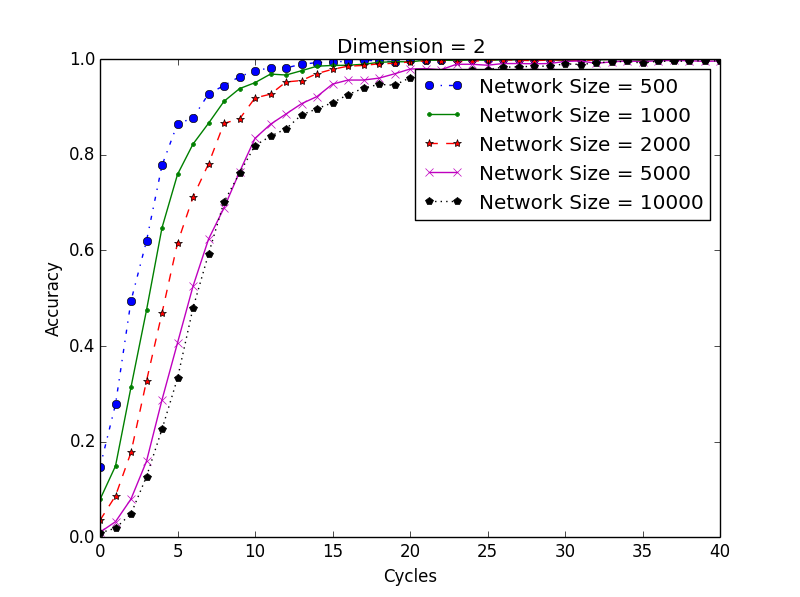
\includegraphics[width=\columnwidth]{conv_d2}
        \caption{This plot shows the accuracy rate of lookups on a 2-dimensional VHash network as it self-organizes.}
        \label{conv2}
\end{subfigure} &

\begin{subfigure}{\columnwidth}
        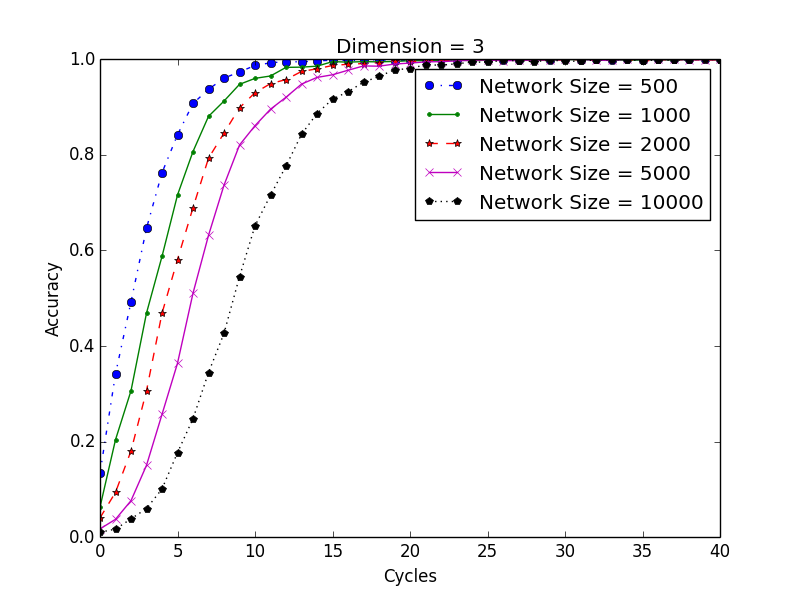
\includegraphics[width=\columnwidth]{conv_d3}
        \caption{This plot shows the accuracy rate of lookups on a 3-dimensional VHash network as it self-organizes.}
        \label{conv3}
\end{subfigure} \\

\begin{subfigure}{\columnwidth}
        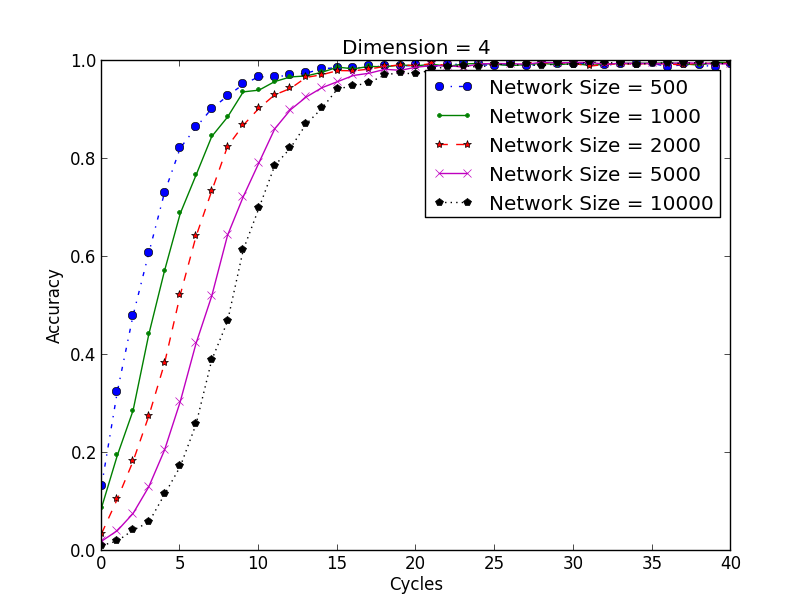
\includegraphics[width=\linewidth]{conv_d4}
         \caption{This plot shows the accuracy rate of lookups on a 4-dimensional VHash network as it self-organizes.}
         \label{conv4}
\end{subfigure} &


\begin{subfigure}{\columnwidth}
        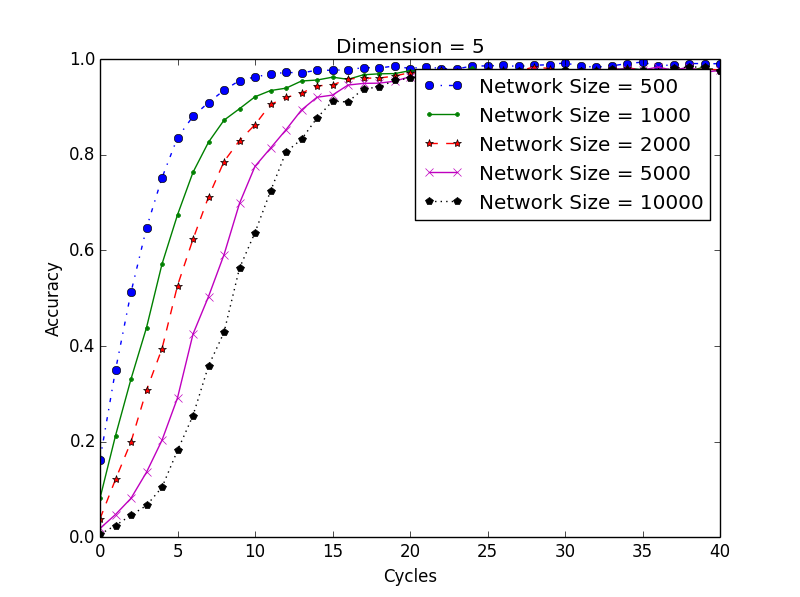
\includegraphics[width=\linewidth]{conv_d5}
                \caption{This plot shows the accuracy rate of lookups on a 5-dimensional VHash network as it self-organizes.}
        \label{conv5}
\end{subfigure}

\end{tabular}

\caption{These figures show that, starting from a randomized network, VHash forms a stable and consistent network topology.
The Y axis shows the success rate of lookups and the X axis show the number of gossips that have occurred.
Each point shows the fraction of 2000 lookups that successfully found the correct destination.}

\end{figure*}
%\begin{table}
%\centering
%\begin{tabular}{|r|r|r|r|}
%\hline
%Network Size & Dimensions & avg degree & max degree\\ \hline
%500   & 2 & 7.004 & 8 \\ \hline
%1000  & 2 & 7.001 & 8 \\ \hline
%2000  & 2 & 7.0015 & 8 \\ \hline
%5000  & 2 & 7.0364 & 66 \\ \hline
%10000 & 2 & 8.0151 & 81\\ \hline  % the heck?
%500   & 3 & 10.364 & 16 \\ \hline
%1000  & 3 & 10.321 & 15 \\ \hline
%2000  & 3 & 10.272 & 16 \\ \hline
%5000  & 3 & 10.3264 & 18 \\ \hline
%10000 & 3 & 9.1233 & 19 \\ \hline
%500   & 4 & x & x \\ \hline
%1000  & 4 & x & x \\ \hline
%2000  & 4 & x & x \\ \hline
%5000  & 4 & x & x \\ \hline
%10000 & 4 & x & x \\ \hline
%500   & 5 & x & x \\ \hline
%1000  & 5 & x & x \\ \hline
%2000  & 5 & x & x \\ \hline
%5000  & 5 & x & x \\ \hline
%10000 & 5 & x & x \\ \hline
%\end{tabular}
%\caption{Information about the size short peer lists, denoted degree here, at the last cycle of the convergence simulation.  For each pair of network size and dimension, we report the average degree in the network, as well as the largest.}
%\label{tab:convtable}
%\end{table}






% Hop distance test
\subsection{Latency Distribution Test}
The goal of our second set of experiments is to demonstrate VHash's ability to optimize a selected network metric: latency in this case. 
In our simulation, we use the number of hops on the underlying network as an approximation of latency.
We compared VHash's performance to that of a more traditional DHT, Chord \cite{chord}.
Chord is a well established DHT with an $O(log(n))$ sized routing table and $O(log(n))$ lookup time measured in overlay hops.  
Rather than examine the number of hops on the overlay network as our primary metric, as done most other analyses of lookup time \cite{kademlia} \cite{chord} \cite{pastry} \cite{raynet} \cite{voronet}, we are concerned with the actual latency lookups experience traveling through the \emph{underlay} network, the network the overlay is built upon.

Overlay hops are used in most DHT evaluations as the primary measure of latency.
It is the best approach available when there are no means of evaluating characteristics of the underlying network.
VHash is designed with a capability to exploit the characteristics of the underlying network.
For most realistic network sizes and structures, there is dramatic room for latency reduction in DHTs.



For this experiment we constructed a 10000 node random scale free network (which has an approximate diameter of 3 hops) as an underlay network \cite{cohen2000resilience} \cite{pastor2001epidemic} \cite{hagberg2004}.
We used a scale-free network as the underlay, as it is a simplified model of the Internet's topology \cite{cohen2000resilience} \cite{pastor2001epidemic}.
From this underlay, we chose a random subset to be members of the overlay network.
We then measured the distance in underlay hops between 10000 random source-destination nodes from the overlay. 
VHash generates an embedding of the latency graph utilizing the distributed force directed model algorithm described in Algorithm \ref{springalg}, with the latency function defined as the number of underlay hops between it and its peers.

Our simulation created 100, 500, and 1000 node overlays for both VHash and Chord.
We used 4 dimensions in VHash and a standard 160 bit identifier for Chord.

\begin{figure}

\begin{subfigure}{\columnwidth}
	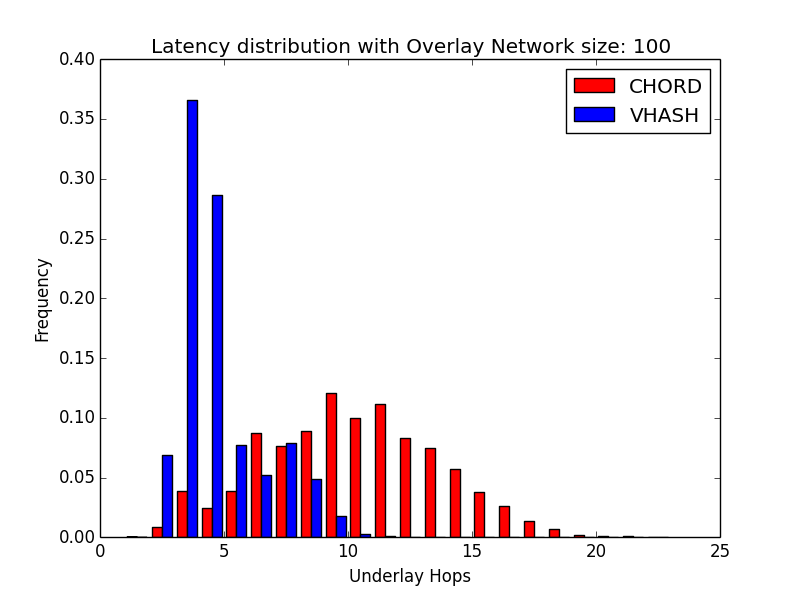
\includegraphics[width=\linewidth]{hist_100}
	\caption{Frequency of path lengths on Chord and VHash in a 100 node overlay.}	
	\label{hist100}
\end{subfigure}

\begin{subfigure}{\columnwidth}
	\centering
	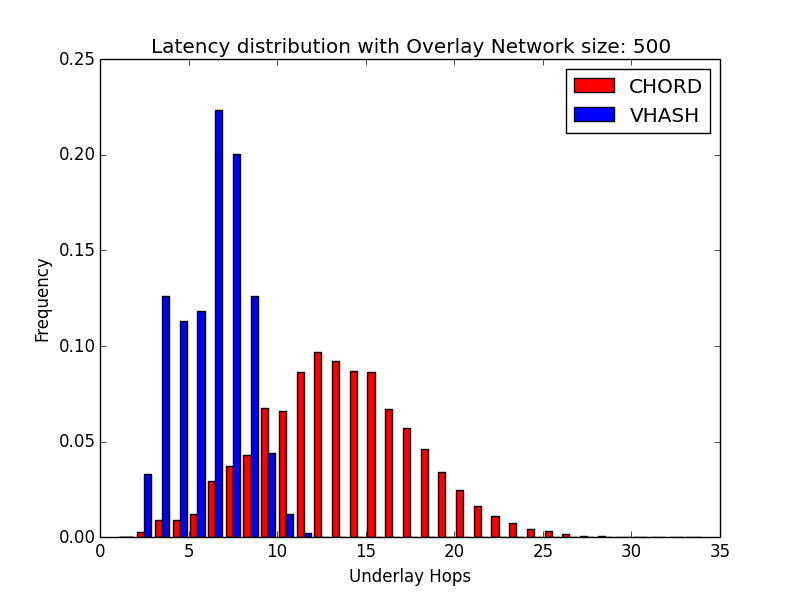
\includegraphics[width=\linewidth]{hist_500}
	\caption{Frequency of path lengths on Chord and VHash in a 500 node overlay.}
	\label{hist500}
\end{subfigure}

\begin{subfigure}{\columnwidth}
	\centering
	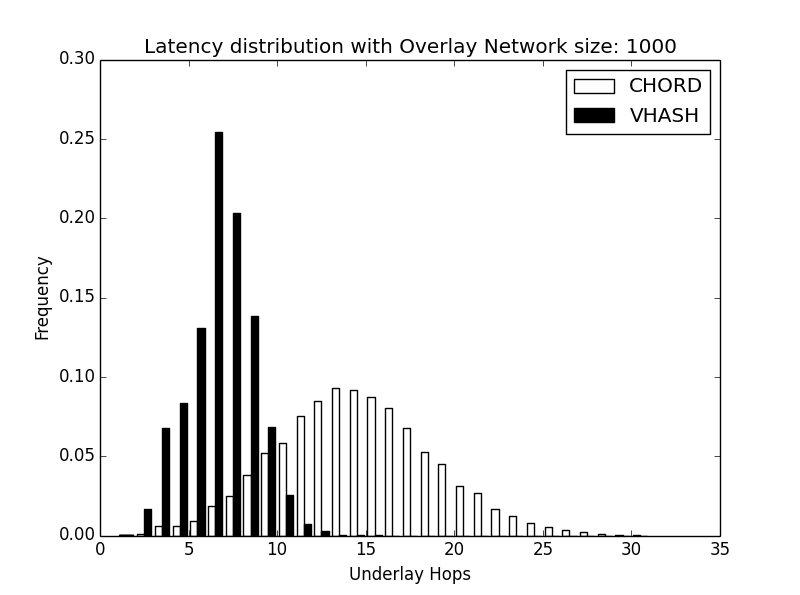
\includegraphics[width=\linewidth]{hist_1000}
	\caption{Frequency of path lengths on Chord and VHash in a 1000 node overlay.}
	\label{hist1000}
\end{subfigure}

\caption{Figures \ref{hist100}, \ref{hist500}, and \ref{hist1000} show the difference in the performance of Chord and VHash for 10,000 routing samples on a 10,000 node underlay network for differently sized overlays. 
The Y axis shows the observed frequencies and the X axis shows the number of hops traversed on the underlay network.
VHash consistently requires fewer hops for routing than Chord.}


\end{figure}



Figures \ref{hist100}, \ref{hist500}, and \ref{hist1000} show the distribution of path lengths measured in underlay hops in both Chord and VHash.   
In all three network sizes, VHash dramatically outperformed Chord and significantly reduced the underlay path lengths.  
Besides having a much lower average path length, the variance was also considerably lower.

For comparison, we also sampled the lookup length measured in overlay hops for a 1000 sized Chord and VHash network.  As seen in Figure \ref{histover}, the paths in VHash's overlay were significantly shorter than those in Chord. 
In comparing the overlay and underlay hops, we find that for each overlay hop in Chord, the lookup must travel 2.719 underlay hops on average; in VHash, lookups must travel 2.291 underlay hops on average for every overlay hop traversed. 
Recall that this work is based on scale free networks, where latency improvements are difficult.
An improvement of 0.4 hops over a diameter of 3 hops is significant.
VHash has on average less overlay hops per lookup than Chord, and for each of these overlay hops we consistently traverse more efficiently across the underlay network.
\begin{figure}[h]
	\centering
	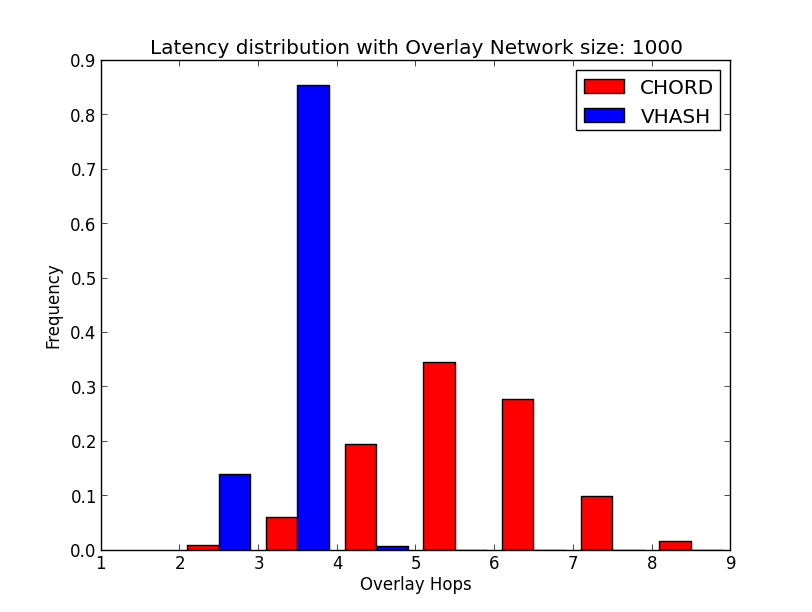
\includegraphics[width=\linewidth]{hist_overlay_4d}
	\caption{Comparison of Chord and VHash in terms of overlay hops.  Each overlay has 1000 nodes.  The Y axis denotes the observed frequencies of overlay hops and the X axis corresponds to the path lengths in overlay hops.}
	\label{histover}
\end{figure}

\section{Related Work}
\label{related}
%check table size consistancy 
While there has been previous work on applying Voronoi regions to DHTs and peer-to-peer (P2P) applications, we have found no prior work on how to perform embedding of an inter-node latency graph.   

Backhaus et al.'s  VAST \cite{Backhaus:2007:VAS:1326257.1326266} is a Voronoi-based P2P protocol designed for handling event messages in a massively multiplayer online video game.  
Each node finds its neighbors by constructing a Voronoi diagram using Fortune's sweepline algorithm \cite{fortune1987sweepline}.  
VAST demonstrated that Voronoi diagrams could be used as the backbone to large-scale applications, although their work focused specifically on using 2-dimensional Voronoi diagrams.  
VHash approximates the Voronoi region rather than solving it, as higher dimension Voronoi regions are computationally expensive to solve.

The two DHT protocols developed by Beumont et al., VoroNet \cite{voronet} and RayNet \cite{raynet} are the closest comparisons to VHash.
VoroNet is based off Kleinberg's small world model \cite{kleinberg2000navigation} and achieves polylogarithmic lookup time.  
Each node in Voronet solves its Voronoi region to determine its neighbors and also maintains a link to a randomly chosen distant node.
Voronet focused specifically on the two-dimensional Voronoi computations and the techniques used would be too expensive in higher dimensions and were not resilient to churn  \cite{raynet}.

RayNet \cite{raynet} was based on the work done on Voronet and is by far the most similar to VHash.  
Like VHash, RayNet does not solve for Voronoi regions, as that is prohibitively expensive.  
RayNet uses a Monte-Carlo method to approximate the volume of a node's Voronoi region.  
While effective at estimating the Voronoi region,  the volume-based Monte-Carlo approximation is expensive and requires multiple samples. 
RayNet does mention the idea of mapping attributes to each axis, but how this can be exploited is left as future work.
 

\section{Conclusions and Future Work}
\label{conclusions}
%\item Explore applications of metric spaces.
Our experiments show that VHash outperforms Chord in overlay-hop latency, underlay-hop latency, and traverses the underlying network more effectively. 
For each overlay hop in Chord, the lookup must travel an average of 2.719 underlay hops per overlay hop.
For each overlay hop in VHash, the lookup instead travels only 2.291 underlay hops per overlay hop on average.
In the context of a scale free graph with an approximate diameter of 3, a difference of 0.4 hops is a significant improvement. 
Further gains in overlay-hop efficiency can be expected from applying VHash with a hyperbolic plane geometric space \cite{papadopoulos2010greedy}.
This would allow for construction of optimally minimal latency networks in VHash.

While we only focus on network latency in this paper as an initial exploration, VHash may be used to optimize multiple network metrics.
These additional metrics can be implemented by mapping them to additional dimensions.
Much of our future work will look at applying VHash to network metrics such as energy or transmission range.
 


%\item Explore file management and backup method.
Another venue for exploration is application of caching and replication strategies to a functional distributed file system running on top of VHash.  Such extensions seek to improve upon existing work done on file replication and caching schemes \cite{shen2010irm}.


%\begin{itemize}
%\item Explore caching and replication strategies.
%\item Find better table sizes?  We kinda just chose ours on an ad-hoc basis
%\end{itemize}



\bibliographystyle{ieeetr}
\bibliography{P3DNS}
\end{document}
